%\documentclass[12pt]{article}
\documentclass[aps,prl,twocolumn,groupedaddress]{revtex4}
%\usepackage{epstopdf-base}
\usepackage{graphicx}
\usepackage{epstopdf}
\usepackage{amssymb}
%\usepackage{wrapfig}
%\usepackage{subfigure}
\usepackage{color}
\usepackage[a4paper, hmargin=2.05cm, vmargin=2.05cm, tmargin=2.05cm, bmargin=5.05cm, nohead]{geometry}
%\documentclass[12pt]{report}
%\documentclass[12pt] {article}
%\renewcommand{\baselinestretch}{2}
%\documentclass[aps,prl,preprint, superscriptaddress]{revtex4}
\renewcommand{\thefigure}{S\arabic{figure}}
%\usepackage{subfigure}
%\usepackage{graphicx}
%\usepackage{afterpage,float}
%\renewcommand{\baselinestretch}{1.2}
\begin{document}
\title{Supplamentary Material for: \\ Thermal analogue of gimbal lock in a colloidal ferromagnetic Janus-rod}

\author{Yongxiang Gao}
\email{yongxiang.gao@chem.ox.ac.uk}
\affiliation{Department of Chemistry, Physical and Theoretical Chemistry Laboratory, University of Oxford}
\author{Andrew Kaan Balin}
\email{andrew.balin@physics.ox.ac.uk}
\affiliation{The Sir Rudolf Peierls Centre for Theoretical Physics, University of Oxford}
\author{Roel P.A.\ Dullens}
\affiliation{Department of Chemistry, Physical and Theoretical Chemistry Laboratory, University of Oxford}
\author{Julia M.\ Yeomans}
\affiliation{The Sir Rudolf Peierls Centre for Theoretical Physics, University of Oxford}
\author{Dirk G.A.L.\ Aarts}
\affiliation{Department of Chemistry, Physical and Theoretical Chemistry Laboratory, University of Oxford}

\date{\today}

\begin{picture}(1,2)
\put(1,2){\line(1,0){8}}
\end{picture}
\maketitle

\subsection*{SM 1. \normalsize Image Analysis}

\begin{figure}[h!]
		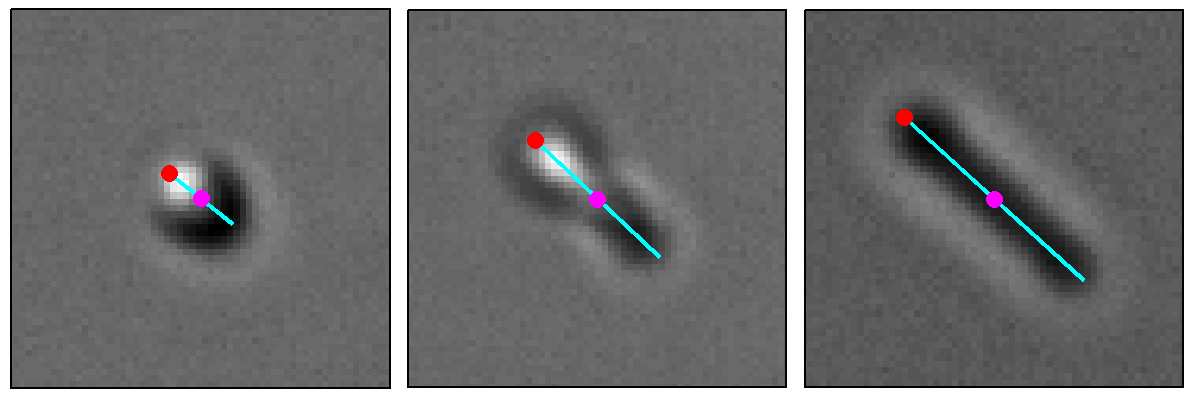
\includegraphics[width=0.95\columnwidth]{figs/FeatureOverlay.png}
	\caption{\footnotesize Reproduction of Fig.\ 2a from Letter.\label{fig}}
\end{figure}

The typical appearances of the rod are shown in Fig.\ \ref{fig}, depending on the relative polar orientation of the body of the rod to the focal plane. We extract the centroid,  length, azimuthal orientation, and the polarity (the magnetic end) of the rod by a Matlab script. Briefly, the background image ($im_b$) averaged over 1000 frames is first removed from the raw images ($im$) to obtain both positive ($im-im_b$) and negative ($im_b-im$) images. A bandpass filter is used to smooth and remove background noise \cite{Crocker1996,Gao2009} from the  images. The positive and negative images are first analyzed separately and binarized by setting an intensity threshold, which is dynamically adjusted such that the smaller dimension of the bounding rectangle of the pixels above the threshold is within the average diameter of the rod ($0.65\pm 0.03 \mu m$) to mitigate the blurring effect from diffraction. The resulted bright and dark pixels above the threshold were then combined together. When the particle appears only dark or bright in the image, the orientation of the particle is determined by approximating these pixels by an ellipse through the ``regionprops'' function of Matlab; otherwise, the orientation is determined by the line linking the centroids of the dark and bright pixels \cite{Gao2009}. The center and length of the particle is set as those of the bounding rectangle of the combined pixels. The last step is to track the polarity of the particle. Minimization of the mean squared displacements of the two ends is used when the particle length ($L_p$) is above a threshold; when $L_p$ is below the threshold, the appearances of the two ends (bright and dark for the ends above and below the focal plane respectively is used \cite{Curtis2002,Lee2007}, which will not change before $L_p$  going above the  threshold. When the rod stays nearly flat on the coverslip, the magnetic end appears slightly bigger and darker due to the presence of magnetite nanoparticles , which is used to distinguish the two ends. Finally, we examine the quality of the image analysis and tracking by overlaying results to the images (SM 2) and correct erroneous ones. 
\bibliography{refs/refs2.bib}

\end{document}
